\documentclass[11pt,a4paper]{article}
\usepackage[utf8]{inputenc}
\usepackage[german]{babel}
\usepackage{amsmath}
\usepackage{amsfonts}
\usepackage{subfig}
\usepackage{amssymb}
\usepackage{siunitx,physics}
\usepackage{mathtools}
\usepackage{graphicx}
%\usepackage{Here}
\usepackage[version=4]{mhchem}
\usepackage{url}
\usepackage{setspace}
\usepackage[left=2.5cm,right=2.5cm,top=2.5cm,bottom=2cm]{geometry}
[biblography=totocnumbered]
\usepackage{fancyhdr}
\usepackage{scrextend}
\usepackage{hyperref}
\pagenumbering{gobble}

\makeatletter
\newcommand\bigcdot{\mathpalette\bigcdot@{.5}}
\newcommand\bigcdot@[2]{\mathbin{\vcenter{\hbox{\scalebox{#2}{$\m@th#1\bullet$}}}}}
\makeatother

\makeatletter
%\renewcommand*\bib@heading{%
%  \subsection*{}%
%  \@mkboth{\refname}{\refname}}
%\makeatother
\numberwithin{equation}{section}
\numberwithin{figure}{section}

\renewcommand{\labelitemii}{\labelitemfont$\vartriangleright$}
\begin{document}\\
\begin{addmargin}[25pt]{0pt}
In polykristallinen Materialien kann es entweder zu einem transgranularem Bruch oder einem intergranularem Bruch kommen. Bei dem transgranularem Bruch breitet sich der Riss unabhängig von den Korngrenzen durch die Körner hindurch aus. Der Riss verläuft entlang spezifischer kristallografischer Ebenen. Beim intergranularem Bruch breitet sich der Riss entlang der Korngrenzen aus, diese Art des Risses entsteht wenn Korngrenzen geschwächt oder versprödet sind. In Abbildung \ref{fig:Rissausbreitung_polykristallin} sind die beiden Rissarten visualisiert.\\
\begin{figure}[h]
    \centering
    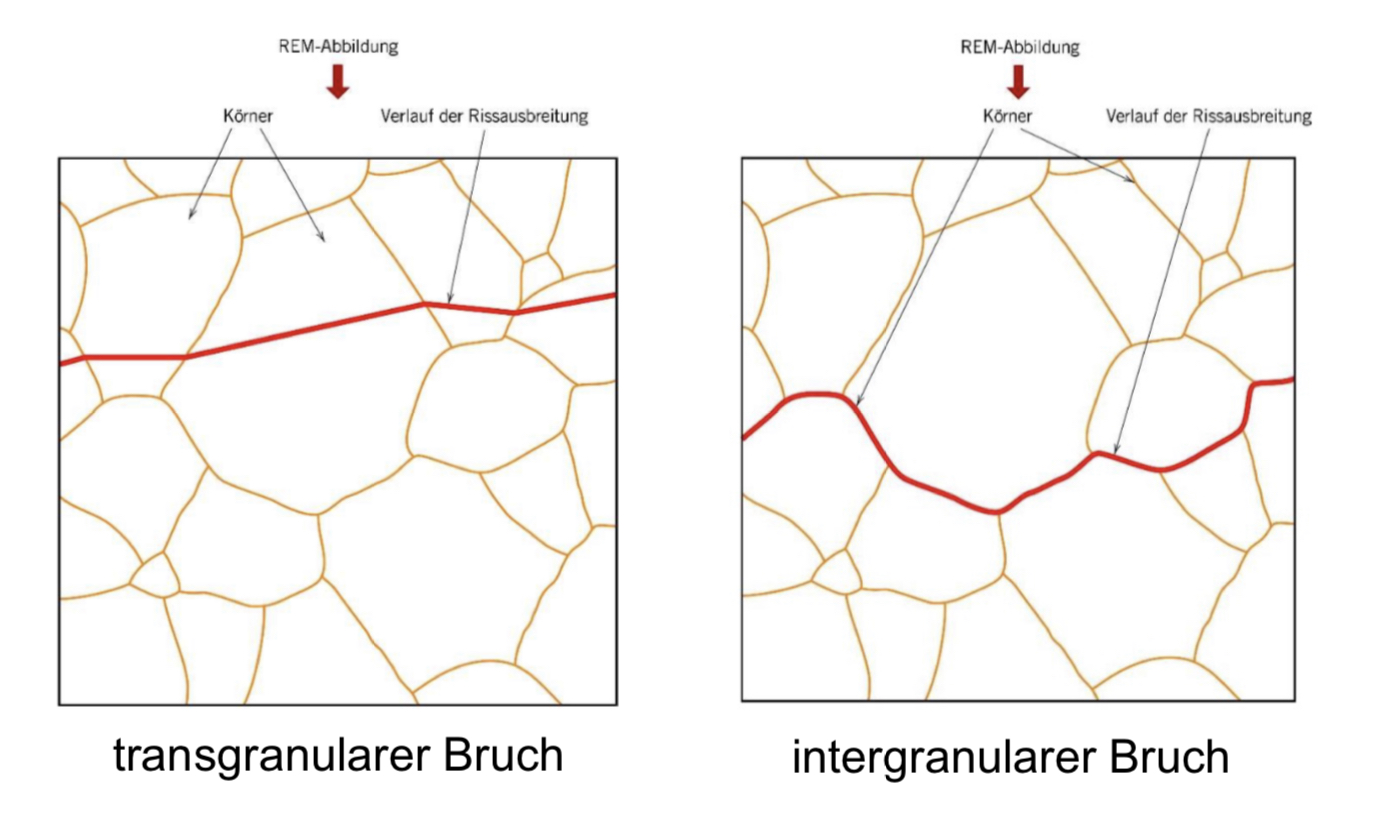
\includegraphics[width = 0.75\textwidth]{images/Materialwissenschaften/Rissausbreitung_polykristallin.jpeg}
    \caption{Darstellung der 2 Arten der Rissausbreitung in polykristallinen Materialien, links der transgrnulare Bruch und recht der intergranulare Bruch.}
    \label{fig:Rissausbreitung_polykristallin}
\end{figure}
\end{addmargin}

\end{document}